\section{Tools \& Technologies}
\subsection*{Languages}
\begin{itemize}
  \item HTML
  \item CSS 
  \item JavaScript 
  \item Python
  \item SQLite3

\end{itemize}
\subsection*{Next.js}
\addcontentsline{toc}{subsection}{Next.js}
\subsection*{FastAPI}
\addcontentsline{toc}{subsection}{FastAPI}
\subsection*{SQLite}
\addcontentsline{toc}{subsection}{SQLite}
\subsection*{Scikit-Learn}
\addcontentsline{toc}{subsection}{Scikit-Learn}
\subsection*{NGINX}
\addcontentsline{toc}{subsection}{NGINX}
\inputminted[fontsize=\footnotesize]{ini}{./codes/nginx.conf}

\subsection*{Docker}
\addcontentsline{toc}{subsection}{Docker}

\begin{figure}[htbp]
  \begin{center}
    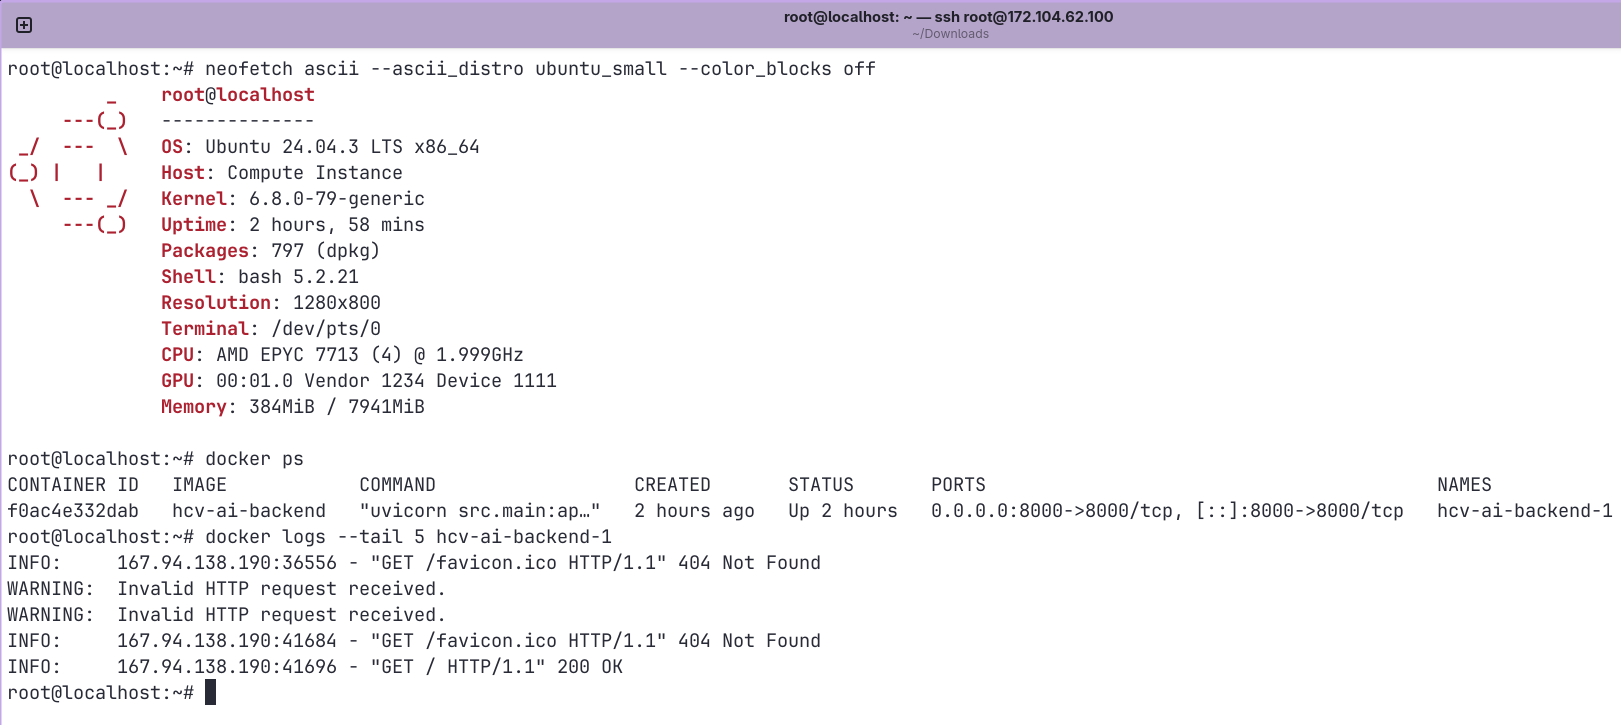
\includegraphics[width=0.95\textwidth]{figures/docker_public_ip.png}
  \end{center}
  \caption{Docker running on linode ubuntu server vps}\label{fig:}
\end{figure}


\section*{Justification for Choice of Technology Stack}

The technology stack for the medical prediction website was carefully chosen to
balance performance, scalability, and ease of development. Next.js was selected
for the frontend because it provides a modern React framework with support
for server-side rendering and static site generation, ensuring fast page loads
and a responsive user interface.

FastAPI\footnote{\url{https://fastapi.tiangolo.com/}} was chosen for the backend due to
its lightweight design, asynchronous capabilities, and automatic API documentation,
which allows for efficient handling of requests and easy integration with machine learning models.

SQLite serves as the database system because it is lightweight, file-based, and easy to set up without
requiring complex configuration, making it well-suited for rapid development and deployment in small to medium-scale applications.

Finally, Scikit-Learn was used for the machine learning component due to its simplicity,
extensive functionality for classification tasks, and seamless integration with Python,
enabling quick development and deployment of the pretrained HCV prediction model.
This combination of technologies ensures that the system is easy to develop, performant,
and maintainable, while also allowing for future migration to more scalable databases if the application grows.
